\chapter{Perspectiva Scrum}

Discriminando todas las filosofías generales, como ideologías y concepciones religiosas, podemos decir que hay perspectivas filosóficas o enfoques relacionados, específicamente, al desarrollo de sistemas y de software. Pues, si bien ocurre que ideologías políticas influyen en los desarrolladores, líderes y arquitectos hay ideas más a fines del ámbito de desarrollo de sistemas, ideas que podemos decir que conforman filosofías influenciadoras. Estas influencias son notorias cuando vemos que se toma una decisión de usar una determinada metodología que implementa algunos principios o se siguen determinados principios sin datos empíricos que sostienen su uso ni explicaciones racionales soportadas con evidencia. A veces dichos principios son como sacados de la galera o reflejan expresión de deseos. Tal como sucede cuando se aplican determinadas tecnologías o metodologías como si se tratasen de una moda o de algo aparentemente arbitrario. También esto se puede apreciar cuando escuchamos decir en una reunión de trabajo en equipo que se premiará al individuo que sobresale (filosofía individualista), que “el éxito del grupo está por encima del individual” (perspectiva Ubuntu o cooperativa), escuchamos en una reunión técnica que “el software debe ser libre” (perspectiva Free Software) o que solo se desarrollara software propietario, que “las mejores arquitecturas, requisitos y diseños emergen de equipos autoorganizados” \cite{Beck-2001} (perspectiva ágil); o que “el software es un mundo de objetos” (perspectiva del Paradigma Orientado a Objetos). Las consignas o lemas organizacionales, los mantras personales o institucionales, las visiones empresariales y lineamientos institucionales también son, en muchos casos, una expresión de filosofías que condicionan a las personas y al desarrollo de software. Por ejemplo, en particular, se da con las filosofías del pensamiento sistémico, pensamiento crítico, filosofía ágil, software libre, software abierto o software propietario, que son las principales que en el mundo del desarrollo de software influencian a sus actores. Estas perspectivas filosóficas suelen presentar principios a seguir y estos principio guían algunas metodologías (prácticas y métodos) de desarrollo de sistemas y a gran parte de desarrolladores de sistemas. Aquí nos vamos a centrar en las perspectivas Scrum y Ágil.

\section{Mentalidad y modelos mentales}

Las personas que participan en el desarrollo de sistemas, diseños organizacionales o industrias de software tienen experiencias, creencias, principios, vivencias y valores que repercuten y condicionan el modo en que ellas perciben la realidad de su día a día y, en consecuencia, repercuten y condicionan a su actuar, su forma de hacer, su trabajo y el resultado del mismo, sistemas hombre-máquina o software. Estas ideas, en los gerentes y desarrolladores, son modelos mentales que conforman una mentalidad, o lo que se denomina mindset (Masa Maeda 2012 \footnote{Masa K Maeda es PhD, Founder and CEO de Valueinnova USA (capacitación Scrum). Es el creador de Serious LeAP, consultor senior del Cutter Consortium en Boston, miembro del comité de dirección del Agile Testing Alliance y maestro en la Universidad de California en Berkeley. Es pionero de Lean y Kanban para trabajo de conocimiento y uno de los formadores del Lean Kanban University. Es una figura líder mundial en Agile y ha generado Serious Games de alto calibre. Previamente hizo I+D para Apple Inc en USA y para Justsystems en Japón. Obtuvo el doctorado y la maestría en Japón.}). O sea que la filosofía o perspectiva filosófica que una persona siga o adhiera está relacionada a los modelos mentales de esa persona y forja su mentalidad o mindset que en algún sentido lo guía.

Los modelos mentales pueden definirse como: “imágenes internas, que están profundamente arraigadas, de cómo funciona el mundo, imágenes que nos limitan a las formas familiares de pensar y actuar”. Los modelos mentales abarcan cuestiones acerca de cómo vemos el mundo y de cómo actuamos en el mundo. 

Tener noción de los modelos mentales es importante para entender que hay detrás de las acciones, de las prácticas y de las metodologías usadas. Nos ayuda a comprender que para realizar cambios en las acciones de las personas y cambios en la forma de hacer las cosas es necesario, la mayoría de las veces, cambiar la mentalidad. Sin cambio de mentalidad puede hacerse insostenible en el tiempo un cambio de hábito, práctica o metodología. Por ese motivo, seguir principios en forma mecánica o por obediencia a la autoridad no forma convicción, y seguir una filosofía sin convicción es un primer condicionante de fracaso práctico en su implementación.

\section{Principios}

En la industria de sistemas y software los principios son reglas, proposiciones o normas que funcionan como máximas o preceptos que orientan la acción. O sea que un principio es como “una regla general de conducta o comportamiento” \cite{Lawson-Martin-2008} \cite{SEBoK-2014}. Un principio es como una recomendación sin el cómo se sigue la recomendación. Cómo hará para seguir la recomendación depende de usted o de quien decida seguir el principio. Por eso son la base, origen y razón fundamental sobre la cual se procede o discurre en materia de sistemas. Se suele usar en el contexto de procesos de desarrollo y metodologías como proposición que da razón, punto de partida o guía, como fundamento de un conjunto de prácticas, una metodología o paradigma de trabajo siendo las metodologías las encargadas de definir el cómo se implementan.

Cada uno sigue algunos principios en su vida como: "trabajo colaborando". También seguimos principios éticos como: “nunca mentir” o “no robar”. A semejanza de los principios éticos tradicionales, ocurre que los principios no necesariamente tienen fundamento objetivo, racional, empírico o basado en evidencias; pues, en ocasiones se comportan más como principios filosóficos que como principios científicos. Lo cual no quiere decir que no deba buscarse que los principios en ingeniería no sean sacados de la galera o usados de forma irracional, sin justificativo razonable y sin comprobación. Es preferible aplicar principios de comprobada efectividad en su aplicación. El aplicar principios comprobados reduce la cantidad de tiempo necesaria para crear las salidas de planificación de los recursos humanos y mejora la probabilidad de que la planificación sea efectiva \cite{PMBOK-2004}, del mismo modo aplicar principios comprobados en actividades de desarrollo y diseño de sistemas reduce tiempos de investigación para generar la salida deseada y minimiza riesgos, mejorando la probabilidad de que el desarrollo sea efectivo. 

Los principios de Scrum son las pautas básicas para aplicar el marco de Scrum y guía a usarse en todos los proyectos Scrum \cite{SBOK-2013}, proyectos en los que se aplica metodología Scrum. Los principios de Scrum se orientan a la gestión de proyectos, desarrollo de productos, trabajo en equipo y el trabajo en base a los principios ágiles. O sea que los principios Scrum tienen correlación con los principios ágiles en forma prácticamente directa \cite{Agile-Atlas-2012}. Y los principios de Scrum están alineados a los valores de Scrum que son: Foco, Coraje, Apertura, Compromiso y Respeto.


A continuación se describen los principios y valores del Manifiesto Ágil y de Scrum.

\section{Manifiesto Ágil}

Los principios del desarrollo ágil se encuentran en el Manifiesto por el Desarrollo Ágil de Software o Manifiesto Ágil [Manifesto Agile 2001], el que expone valores y principios firmado por diecisiete personas convocadas por Kent Beck \cite{Beck-2001}. Los principios del desarrollo ágil surgieron como principios base y originarios de métodos que estaban surgiendo como alternativa a las metodologías clásica formales (CMMI, SPICE, etc.) a las que, autores como Kent Beck, consideraban excesivamente pesadas y rígidas por su carácter normativo y fuerte dependencia de planificaciones detalladas completas y previas al desarrollo \cite{Wiki-2015}.

\subsection{Valores del Manifiesto Ágil}

El Manifiesto Ágil propone los siguientes valores:

\begin{enumerate}

\item \textbf{Individuos e interacciones sobre procesos y herramientas:} hay que priorizar la confianza puesta en los equipos, los individuos dentro de esos equipos y la manera en que éstos interactúan, en vez de seguir rígidamente procesos y herramientas. Pues, son los equipos quienes deben resolver qué hay que hacer, cómo hay que hacerlo y finalmente son ellos quienes lo hacen. Pues los equipos no deberán ser meros autómatas que reciben órdenes jerárquicas de la organización de arriba hacia abajo sino que, en lugar de eso, se espera que de abajo hacia arriba sepan resolver los problemas, ofrecer sus propios métodos de trabajo y ser hasta cierto punto autosuficientes. En este sentido, hay que delegar en ellos la identificación de qué se interpone en el camino de sus metas y la asunción de la responsabilidad de buscar resolver todas las dificultades que se encuentren dentro de su alcance. Se les debe permitir trabajar en conjunto con otras partes de la organización para resolver asuntos que están más allá de su control.

\item \textbf{Software funcionando sobre documentación extensiva:} hay que estar orientado al producto o focalizarse en él y, de este modo, requerir un incremento de producto completo y funcionando como resultado final de cada ciclo de trabajo, en vez de tener que cumplir con grandes y engorrosas documentaciones y formalismos burocráticos. Ciertamente, en la construcción del producto, es necesario realizar determinada documentación, pero es el producto concreto o funcionando lo que permite a la organización guiar al proyecto hacia el éxito. Es crucial que los equipos produzcan un incremento de producto en cada ciclo de trabajo.

\item \textbf{Colaboración con el cliente sobre negociación contractual:} en vez de tener comunicación pobre debido a restricciones contractuales, el cliente debería ser el punto de contacto principal del equipo, en colaboración de trabajo, con los eventuales usuarios finales del producto y con las partes de la organización que necesitan el producto. Se debería ver al cliente como un miembro del equipo que trabaja colaborativamente con el resto de integrantes para decidir qué debe hacerse y qué no. Con el cliente se debería poder seleccionar el trabajo que debe realizarse a continuación, asegurando que el producto tenga el valor más alto posible en todo momento. Esto es crucial, construir una fuerte colaboración con el cliente en vez de negociar contratos rígidos que obstaculizan el trabajo ágil y generan fricción con el cliente.

\item \textbf{Respuesta ante el cambio sobre seguir un plan:} el avance del trabajo o del equipo debería estar representado por un incremento de producto real y que funciona, y no por una correcta correlación y contrastación a un plan. Se debe priorizar la flexibilidad para adaptación a cambios en vez de la rigidez de seguir un plan detallado. Para ello, los equipos deberían inspeccionar lo que sucede de forma abierta y transparente buscando adaptar sus acciones a la realidad. O sea que, la planificación se debería adaptar a la realidad y al equipo y no al revés.

\end{enumerate}

Se puede notar que estos valores son aplicables a cualquier tipo de organización e industria. Pues, solo el segundo valor se refiere particularmente a la industria de software y el mismo se puede reformular de forma más general como sigue: trabajar orientados al producto funcionando más que sobre una amplia y extensa documentación \cite{Sriram-Narayan-2015}.

\subsection{Principios del Manifiesto Ágil}

Alineados a estos valores, el Manifiesto Ágil propone los siguientes principios:

\begin{enumerate}

\item \textbf{Entregar valor temprano y continuamente:} Nuestra mayor prioridad es satisfacer al cliente mediante la entrega temprana y continua de software con valor. Tratamos de entregar lo más rápido posible valor funcional.

\item \textbf{Apertura al cambio:} Aceptamos que los requisitos cambien, incluso en etapas tardías del desarrollo. Los procesos Ágiles aprovechan el cambio para proporcionar ventaja competitiva al cliente.

\item \textbf{Entregables frecuentes:} Entregamos software funcional frecuentemente, entre dos semanas y dos meses, con preferencia al periodo de tiempo más corto posible.

\item \textbf{Cooperación con el cliente:} Los responsables de negocio y los desarrolladores trabajamos juntos de forma cotidiana durante todo el proyecto, potenciando de esta manera al equipo. O sea que se privilegia una cooperación constante entre miembros del equipo e interesados externos al equipo (como clientes).

\item \textbf{Personas motivadas:} Los proyectos se desarrollan en torno a individuos motivados. Hay que darles el entorno y el apoyo que necesitan, y confiarles la ejecución del trabajo. Un equipo que es libre de decidir sobre cómo hacer su trabajo y trabaja en un ambiente de seguridad psicológica, es bastante probable que sea un equipo motivado.

\item \textbf{Conversación cara a cara:} El método más eficiente y efectivo de comunicar información al equipo de desarrollo y entre sus miembros es la conversación cara a cara. La priorización de conversar en persona, por sobre las conversaciones diferidas, acelera la toma de decisiones y la solución de impedimentos.

\item \textbf{Orientación al producto:} El producto funcionando es la medida principal de progreso. Es más importante que un producto funcione como se espera más que cumplir con un hito, medirlo o documentarlo.

\item \textbf{Desarrollo sostenible:} Los procesos Ágiles promueven el desarrollo sostenible. Los promotores, desarrolladores y usuarios debemos ser capaces de mantener un ritmo constante de forma indefinida.

\item \textbf{Excelencia técnica:} La atención continua a la excelencia técnica y al buen diseño mejora la agilidad.

\item \textbf{Simplicidad eficiente:} La simplicidad, o el arte de maximizar la cantidad de trabajo no realizado, es esencial (alineado al principio de simplicidad). Este estilo de prácticas es parte de algo que, en metodologías ágiles, se conoce como: "hacer todo lo posible por hacer lo menos posible" \cite{Anacleto-2005}. Por ejemplo en Arquitectura se puede considerar mantener una lo más simple posible. Si la simpleza se traduce en facilidad de uso de la arquitectura, facilidad para entender los conceptos involucrados y documentación necesaria, es muy probable que el nivel de productividad aumente \cite{Anacleto-2005}. En este sentido la simpleza de la arquitectura es un requerimiento de calidad alineado a la filosofía ágil.

\item \textbf{Equipos auto-organizados:} Las mejores arquitecturas, requisitos y diseños emergen de equipos auto-organizados (alineado al principio sistémico de emergencia). Los equipos auto-organizados son aquellos que tienen proactividad y autonomía para tomar decisiones de producción y gestión, como también así la de ejercer la auto-regulación mediante el monitoreo y control de sus actividades y resultados. Estos equipos tienen mayor libertad para crear.

\item \textbf{Equipos auto-reflexivos:} A intervalos regulares el equipo reflexiona sobre cómo ser más efectivo para, a continuación, ajustar y perfeccionar su comportamiento en consecuencia. Los equipos auto-reflexivos son los que evolucionan por medio de procesos de mejora continua constante.

\end{enumerate}

\subsection{Corazón de la agilidad}

Como se observa anteriormente, los valores y principios suman 16 incisos y son bastantes para ser recordados facilmente. Para ayudar en su aprendizaje, se puede recurrir a unificarlos en un mandala ágil con los cuatro conceptos claves, corazón de la agilidad: colaboración, orientación a la entraga, adaptación y mejora continua (ver fig. \ref{fig:MandalaAgil}).

\begin{figure}[h]
  \centering
  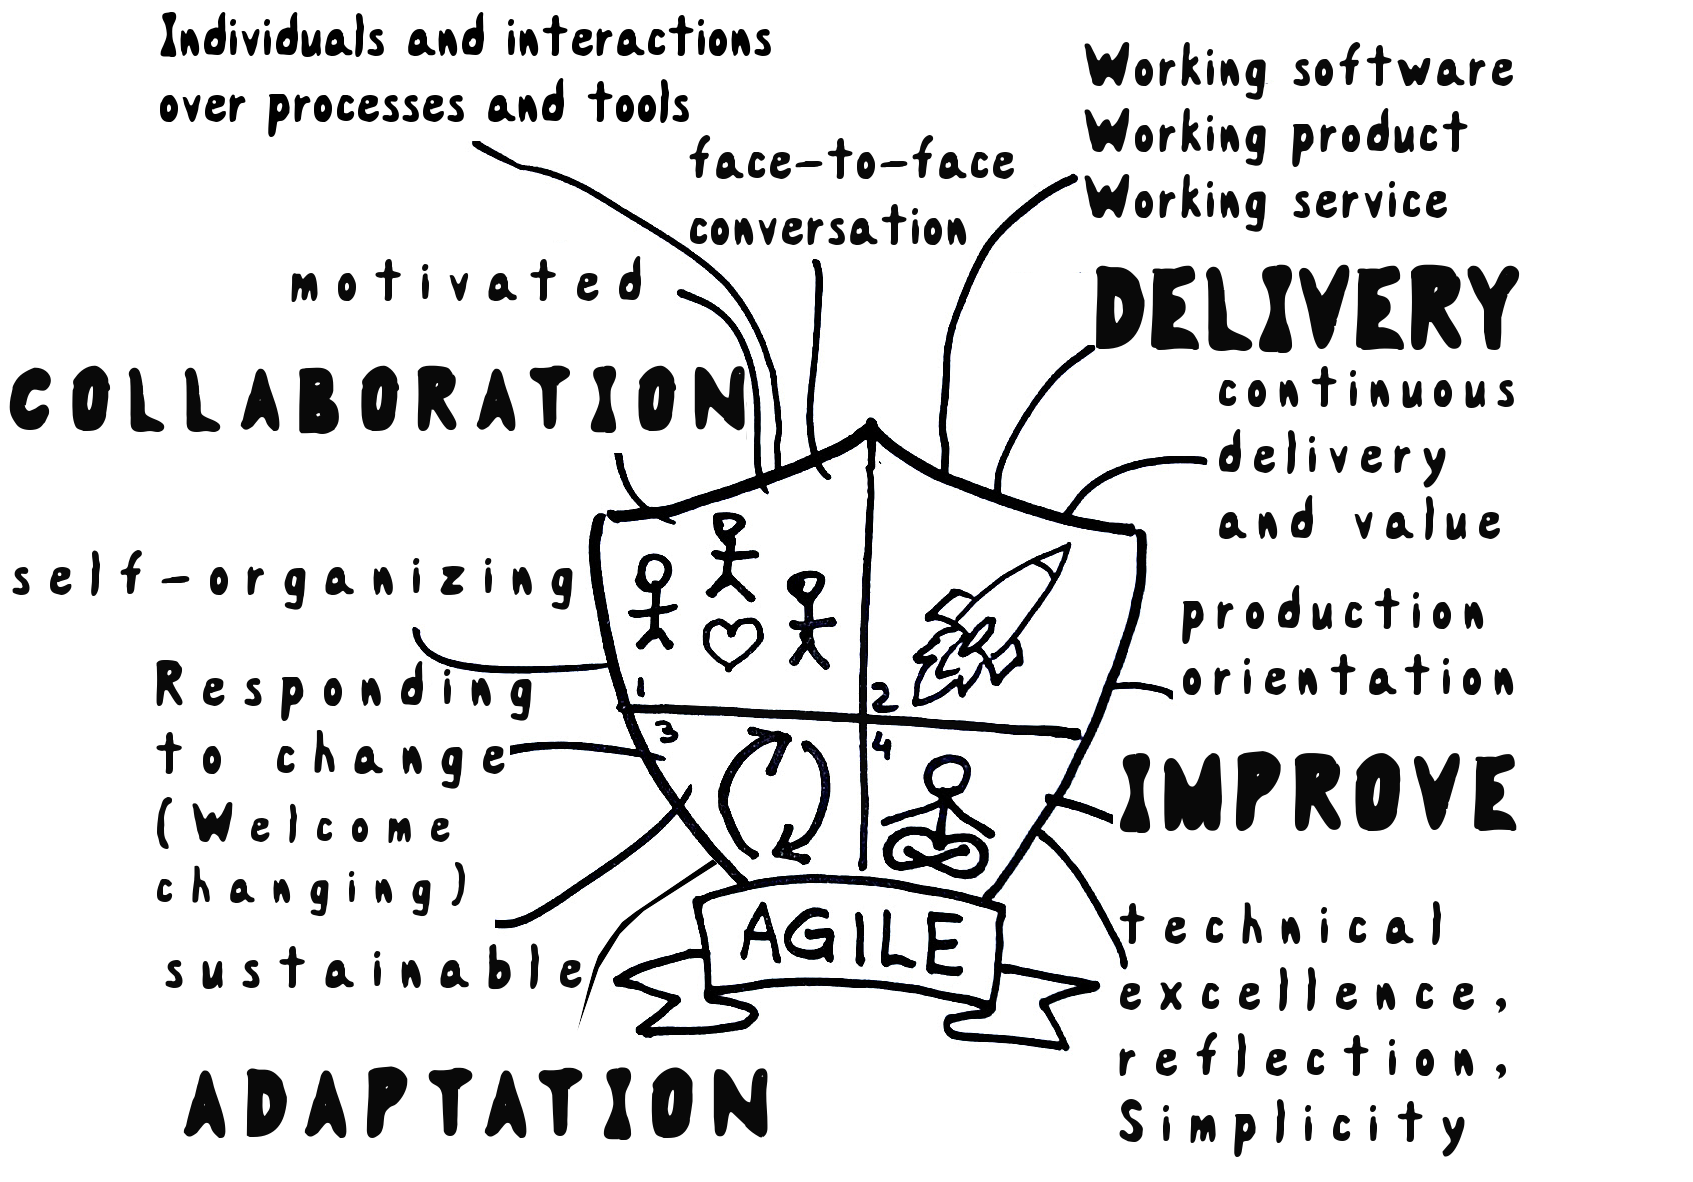
\includegraphics[width=0.99\textwidth]{MandalaAgil}
  \caption{Mandala ágil}
  \centering
  \label{fig:MandalaAgil} %\ref{fig:MandalaAgil}
\end{figure}

\section{Valores de Scrum}

El corazón de Scrum es el control empírico sostenido por la transparencia, la inspección y la adaptación\footnote{\cite{Ken-Jeff-2013}}. Aunque, sin embargo, la Scrum Alliance propuso cinco valores esenciales a seguir\footnote{\cite{Scrum-Alliance-2015}}: 

\begin{enumerate}
\item \textbf{Foco:} hay que enfocarse en sólo unas pocas cosas a la vez, trabajamos bien juntos y buscando producir un resultado excelente tratando de entregar ítems valiosos en forma pronta. Si bien Scrum no prescribe ninguna especificación de foco, podemos entender como foco a: no desviarse del objetivo del producto y de iteración, buscar hacer historias (PBIs) alineadas al objetivo de la iteración primero, hacer las tareas más prioritarias y en progreso, mantener el trabajo en progreso con una cantidad de trabajo óptima para el equipo en la iteración, desarrollar conversaciones sin ruido comunicativo, ordenada, y hacer que las ceremonias y reuniones sean eficaces, manteniendo el foco en el objetivo de la reunión y en su éxito.

\item \textbf{Coraje:} hay que buscar sentirse apoyados y tener más recursos a disposición para promover el coraje para enfrentar desafíos más grandes. Además, para poder lograr cambios significativos en una organización que mantiene una cultura con principios y valores que entran en conflicto con los de Scrum y el Manifiesto Ágil, es necesario tener coraje para impulsar el cambio y plantarse en forma efectiva ante la resistencia al cambio. En este sentido, coraje se refiere al valor que hay que tener para no dejarse dominar ante la idiosincrasia predominante y el “status quo” que atentan contra el pensamiento Scrum.

\item \textbf{Apertura:} Hay que tener apertura para expresar cotidianamente cómo nos va, qué problemas encontramos, manifestar las preocupaciones y aceptar las sugerencias de los pares para que éstas puedan ser tomadas en cuenta por nosotros y por los demás. La apertura requiere capacidad de aceptación y tolerancia ante la crítica y la opinión de los demás.

\item \textbf{Compromiso:} Se busca lograr compromiso para el éxito gracias a promover el mayor control nuestro sobre lo que hacemos y nuestro destino. Hay mayor probabilidad de lograr compromiso en las personas que deciden sobre lo que hacen.

\item \textbf{Respeto:} Buscamos convertirnos en merecedores de respeto a medida que trabajamos juntos, compartiendo éxitos y fracasos, llegando a respetarnos los unos a los otros y ayudándonos mutuamente.
\end{enumerate}

\section{Principios de Scrum}

Se suele asociar a los valores del Manifiesto Ágil como principios de Scrum. Por lo que, en primera instancia, los cuatro valores ágiles son los principales principios de Scrum. Pero para no repetirlos en esta sección vamos a nombrar otros seis principios que en diferente bibliografía se suelen atribuir a Scrum. Los mismos son:

\begin{enumerate}

\item \textbf{Control Empírico:} El proceso empírico de control del proyecto es más efectivo que el control predictivo de largos plazos. Es más efectivo para gestionar la complejidad y obtener el mayor valor posible, basado en inspección y adaptación regular en función de los resultados que se van obteniendo y del propio contexto del proyecto (auto-regulación). El proceso empírico permite adaptabilidad a requisitos que emergen del mismo proceso de desarrollo. Con este principio como marco, podemos usar metodologías, prácticas, técnicas y ser nosotros (o el propio equipo de trabajo) los que a través del empirismo, determinemos la forma más adecuada de hacer las cosas para lograr los objetivos. Son los equipos de desarrollo los que deben hacer lo que sea necesario para entregar el producto esperado y aprender de su propia experiencia mediante exploración y experimentación \cite{UNTREF-2014}. Es el equipo el que determina qué prácticas y herramientas les dan los mejores resultados, y así mejoran de manera continua. Los buenos equipos trabajarán constantemente en mejorar y aprender de sus experiencia. Además, se debe aprender de la experiencia de los demás leyendo libros y buscando la experiencia de personas que ya hayan venido probando algunas prácticas, o que están experimentando con nuevas potenciales mejores formas de hacer las cosas a través de la inspección y la adaptación. 

\item \textbf{Auto-organización:} Los equipos auto-organizados pueden auto-gestionarse y de ellos emerge la sabiduría necesaria para la gestión de sus proyectos y actividades, y así lograr la sinergia necesaria para resolver problemas en forma ágil. Esta idea proviene de la concepción de que de un sistema social puede emerger inteligencia de grupo como puede suceder en una bandada de pájaros. Esta es una premisa aceptada en Inteligencia Artificial, pensamiento sistémico y en filosofía emergentista. Se considera que en un sistema con agentes inteligentes, a partir de reglas locales simples puede emerger inteligencia grupal colectiva o de enjambre, pues se considera que la "información local puede conducir a la sabiduría global" \cite{Steven-Johnson-2002}. De aquí que, de la auto-organización en equipos de trabajo puede surgir inteligencia o también sabiduría según un fenómeno conocido como "sabiduría de multitud" o "wisdom of the crowd" \cite{MIT-Press-2009} en la que la opinión colectiva de un grupo puede ser mejor que la individual de un experto. Este fenómeno, no sólo es útil a la gestión de proyectos, sino también a las actividades de estimación, pues el promedio de muchas estimaciones individuales suele estar mucho más cerca del valor real que la estimación de un experto. En lo referente al diseño se cree, como lo indica el principio 11 (once) del Manifiesto Ágil, que se logran mejores diseños y arquitecturas desde equipos auto-organizados \cite{UNTREF-2014}. En lo referente al liderazgo se cree que no es necesario un líder jerárquico, autoritario o experto que guíe al equipo sino que es el propio equipo el que genera su liderazgo. Según esta perspectiva se puede prescindir de la figura de líder tradicional o jefe, se puede carecer de líder, lograr muchos líderes o tener un líder con perfil más bien de facilitador (servicial e integrador).

\item \textbf{Colaboración:} Se puede entender a la colaboración como la capacidad de reconcebir nuestras propias ideas a la luz de la de las demás \cite{Austin-2003} para poder lograr ideas colectivas mejores que las ideas individuales \cite{UNTREF-2014}. Las ideas en colaboración son resultado y mérito del equipo y no de alguno de sus integrantes. La agilidad requiere de colaboración, colaboración interna en el equipo y externa con el cliente. Colaborar con el cliente permite guiar de manera regular los resultados del proyecto de desarrollo. O sea que, la colaboración en el marco de agilidad se orienta directamente a conseguir los objetivos del cliente en un proyecto mediante el trabajo en equipo colaborativo. El trabajo en equipo con colaboración del cliente posibilita su frecuente retroalimentación y mantenerse alineado a su punto de vista y sus expectativas para satisfacer sus necesidades o los requisitos del desarrollo, por el cual el sistema producto se desarrolla con mayor agilidad. La colaboración interna requiere soltura y apertura para dejar los egos de lado e integrarse en el proceso de pensamiento colectivo, donde los problemas los resuelven todos los del equipo con sus aportes individuales. En el marco de colaboración se dejan de lados los héroes, pues los héroes no ven el gran dragón Malveau 2004 y los héroes se suelen llevar los créditos. La cooperación es la convicción de que nadie llega a la meta si no llegan todos (Virginia Burden).

\item \textbf{Priorización por valor:} Se prioriza por valor, es decir que se puede ser más efectivo si se hacen primero las tareas que suman más valor al negocio o a las necesidades del cliente. Se hace necesario prescindir de requisitos de baja prioridad antes que tener que degradar la calidad.

\item \textbf{Limitación de tiempos (time-boxing):} El trabajo limitado en periodos de tiempo ayuda en la regularidad en las actividades. Por eso, las iteraciones de trabajo, las actividades y las reuniones deben tener un límite de tiempo y se debe buscar no sobrepasar esos límites.

\item \textbf{Desarrollo iterativo:} El desarrollo iterativo permite una construcción gradual en proyectos complejos. En cada iteración el equipo evoluciona el producto (hace una entrega incremental) a partir de los resultados completados en las iteraciones anteriores, añadiendo nuevos objetivos/requisitos o mejorando los que ya fueron completados, de manera que el cliente pueda obtener los beneficios del proyecto de forma incremental. El desarrollo iterativo permite gestionar las expectativas del cliente (requisitos desarrollados, velocidad de desarrollo, calidad) de manera regular y lograr reacción, aceptación del mercado y adaptabilidad. Permite que el cliente pueda obtener resultados importantes y útiles ya desde las primeras iteraciones. Facilita la mejora ya que al tener experiencias por períodos de iteración se puede mejorar de las experiencias de iteraciones previas y permite planificar los cambios necesarios para aumentar la productividad y calidad en iteraciones subsiguientes.

\begin{figure}[h]
  \centering
  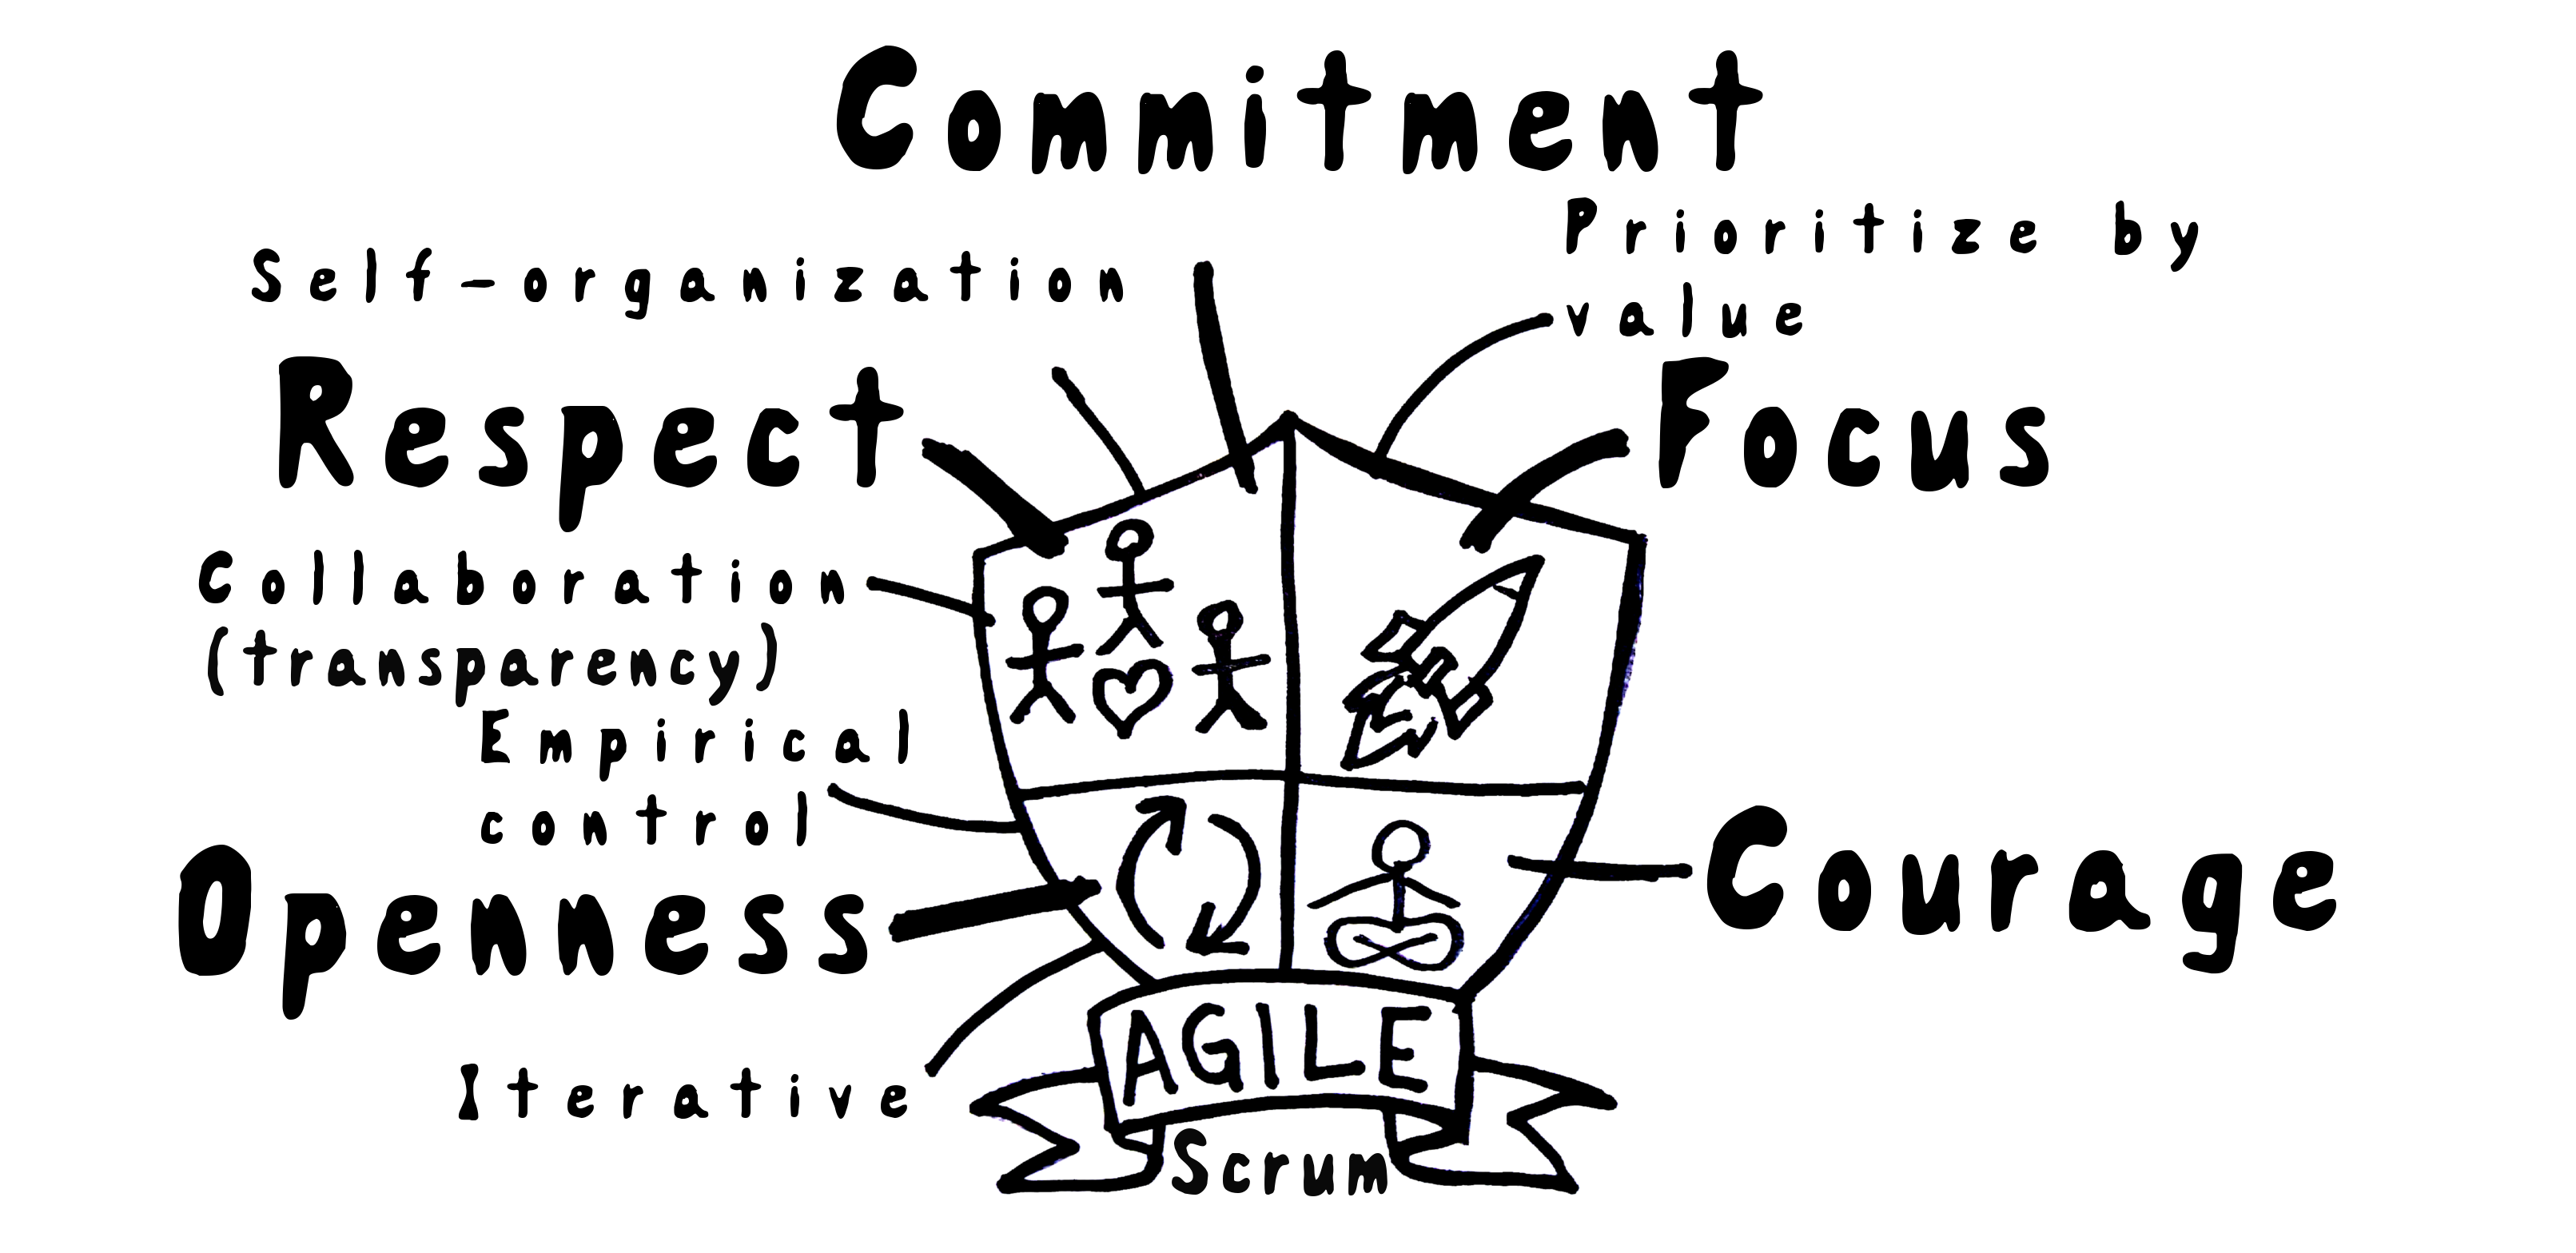
\includegraphics[width=0.99\textwidth]{MandalaAgilScrum}
  \caption{Mandala ágil para Scrum}
  \centering
  \label{fig:MandalaAgilScrum} %\ref{fig:MandalaAgil}
\end{figure}

\end{enumerate}

\section{Ideas filosóficas relacionadas}

\subsection{Emergentismo}

Scrum adhiere al principio de auto-organización y está alineado al Manifiesto Ágil y a su filosofía. En la filosofía ágil se toma una idea basada en el emergentismo que la podemos encontrar en el principio: "Las mejores arquitecturas, requisitos y diseños emergen de equipos auto-organizados" \cite{Beck-2001}. El emergentismo sostiene que el "todo puede ser más que la suma de las partes"\footnote{"The whole is more than the sum of its parts" (Ludwig Von Bertalanffy, General System theory, 1968). Esta idea del sistemismo y el emergentismo también está relacionada al holismo que sostiene la misma afirmación.} que significa que desde un nivel de realidad dado (n) donde componentes se interrelacionan (S1, S2, S3... Sn) pueden emerger sistemas, propiedades o características nuevas en el nivel superior (n+1) que no existen en los componentes individuales, pero que relacionados la generan (ver figura \ref{fig:Emergentism}). En este sentido suele llamarse emergencia al fenómeno en el que algo emerge o es emergente, en el que una totalidad nueva llega a existir, a una cosa nueva que posee una propiedad emergente, a un proceso nuevo que surge de algo, a una estructura que aparece de otras, a un orden que viene de otro, a una novedad cualitativa en la naturaleza que brota, a un sistema que resulta de componentes relacionados o al surgimiento espontáneo de algo nuevo.

\begin{figure}[h]
  \centering
  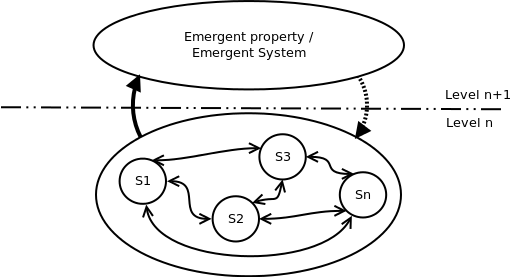
\includegraphics[width=0.9\textwidth]{Emergentism}
  \caption{Modelo de emergentismo}
  \centering
  \label{fig:Emergentism} %\ref{fig:Emergentism}
\end{figure}

En este sentido, la auto-organización sucede cuando componentes, sistemas o personas se organizan sin aparente dirección o mando controlador y generan espontáneamente una forma global de orden o coordinación. Esto se da en una gran variedad de fenómenos físicos, químicos, biológicos, sociales y sistemas cognitivos. A nosotros nos incumbe principalmente lo relacionado a lo social e informático. 

\subsection{Sinergia}

En lo social se sabe que se pueden lograr equipos de personas con una alta organización y coordinación sin la necesidad de un líder director, sin un líder que ordene y controle, e incluso sin planificación alguna. Pues, no solo organización y coordinación se puede lograr desde equipos auto-organizados, sino que también se puede lograr sinergia. La sinergia es la prestancia extra que puede dar un equipo debido a la acción conjunta de individuos en equipo que es superior a la suma de las individualidades. Otra propiedad emergente que se puede lograr en grupos auto-organizados es la inteligencia colectiva o inteligencia enjambre que incluye a la "Ley de Linus" y a la "Sabiduría de grupo".

\subsection{Ley de Linus}

Se pueden formar muchos tipos de inteligencia colectiva en equipos colaborativos. Por ejemplo, lo más común en el desarrollo de software es que problemas extremadamente complejos sólo pueden ser resuelto por un conjunto de personas trabajando conjuntamente en él, a pesar de que muchas veces sea una sola persona la que resuelva un determinado problema, esa persona nunca podría haberlo hecho sola. Es decir que, dada una base suficiente de desarrolladores y testers validadores colaborando, casi cualquier problema puede ser caracterizado rápidamente, y su solución ser obvia \cite{Eric-Raymond-1997}. A esta idea de inteligencia colectiva se la denomina "Ley de Linus".

\subsection{Sabiduría de multitud}

La Sabiduría de grupo o de multitudes es una idea, apoyada en evidencias, de que dada "ciertas condiciones" las decisiones o predicciones tomadas colectivamente por un grupo de personas suelen ser más atinadas que las decisiones o predicciones individuales o que las que son tomadas sobre la base del conocimiento de un experto \cite{James-Surowiecki-2005}\footnote{"The wisdom of the crowd is the collective opinion of a group of individuals rather than that of a single expert." \cite{MIT-Press-2009}}. Es más, a medida que el grupo es más grande, las decisiones o predicciones son más acertadas.

Claro que para que esto suceda deben cumplirse ciertas condiciones. Para Surowieki (escritor del libro La Sabiduría de las Multitudes\footnote{\cite{James-Surowiecki-2005}}) las condiciones necesarias son:

\begin{enumerate}

\item \textbf{Diversidad:} el grupo debe tener diversidad de perfiles para lograr una diversidad de Opiniones. Pues, si todos los del grupo piensan igual o semejante, pertenecen a la misma tribu urbana o subcultura, son de la misma profesión o tienen las mismas características de perfil profesional o psicológico, entonces es menos probable de que logren una sabiduría de grupo.

\item \textbf{Independencia:} el grupo no debería estar influenciado y las opiniones de los integrantes tampoco. Si las personas son influenciadas por el grupo se puede caer en lograr el "pensamiento de grupo" y tomar decisiones malas o irracionales. Por otro lado, si el grupo es influenciado por un actor externo al grupo, la decisión grupal es dirigida y, hasta en algún sentido, manipulada.

\item \textbf{Agregación:} El sistema de decisión grupal debe ser agregativo, que significa que debe tener la capacidad de sumar o promediar las opiniones individuales. Un sistema de votación no agregativo, por ejemplo por votación de la mayoría sobre una alternativa, puede hacer prevalecer una decisión individual. Un ejemplo de agregación es cuando la decisión métrica grupal se basa en el promedio de todas la decisiones\footnote{Un ejemplo de Sabiduría de multitud es cuando se le pide a muchas personas que predigan la cantidad de elementos contenidos en un frasco transparente. Es sorprendente como el promedio se acerca considerablemente al número real.}.


\item \textbf{Pericia:} Yo agregaría pericia. Pues, si juntamos a un montón de filósofos, escritores y médicos a estimar una tarea de desarrollo de software, es muy probable que fallen en hacerlo por no tener idoneidad.
 

\end{enumerate}

\subsection{Arquitectura emergente}

Hay dos formas extremas de ver el desarrollo de software incluyendo al diseño. Una es la que sugiere que se pueden prever todas las cientos de miles de cuestiones que emergen cuando se desarrolla el software y, en consecuencia, se trata de limitar las respuestas a las mismas conduciendo un desarrollo planificado, estructurado, dirigido y liderado (el extremo izquierdo del aspecto que se muestra en la figura \ref{fig:DesignSpectrum}) \cite{Neal-Ford-2010}. La otra forma es no anticipar nada, permitiendo que las soluciones software surgan espontáneamente a medida que evoluciona el desarrollo en un proceso no dirigido, no liderado y descentralizado (el extremo derecho del aspecto que se muestra en la figura \ref{fig:DesignSpectrum}). En la primera opción el rol de los líderes y expertos (por ejemplo líderes de proyecto y arquitectos expertos), las reglas globales de dirección, el trabajo de comienzo y la información inicial es fundamental para el desarrollo. En el lado de la segunda opción, la orientada a fenómenos emergentes, el rol de todos los actores, el trabajo en equipo y las reglas locales de trabajo son lo principal para el desarrollo. La emergencia de la arquitectura se da, entre otras cosas, cuando se crea una arquitectura inicial simple y flexible, con decisiones tomadas que no son irreversibles, y con una evolución en el tiempo que considera a los nuevos requisitos y problemas que surjan.

\begin{figure}[h] 
  \centering
  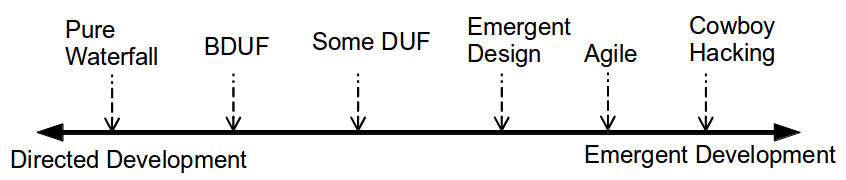
\includegraphics[width=0.99\textwidth]{DesignSpectrum}
  \caption{Modelo del espectro del tipo desarrollo de software}
  (Espectro que abarca el diseño \cite{Neal-Ford-2010})
  \centering
  \label{fig:DesignSpectrum} %\ref{fig:DesignSpectrum}
\end{figure}

Hay una obra literaria llamada "La catedral y el bazar"\footnote{\cite{Eric-Raymond-1997}} escrita por el hacker Eric S. Raymond en 1997 que expone esta idea. La misma analiza dos modelos de producción de software: la catedral que representa el modelo de desarrollo más hermético y vertical (el lado izquierdo de la figura \ref{fig:DesignSpectrum}) y por otro lado el bazar, con su dinámica horizontal y bulliciosa (el lado derecho de la figura \ref{fig:DesignSpectrum}).

\subsection{Resiliencia}

Generalmente no queremos ser frágiles y vulnerables. Y en trabajo de equipos no queremos equipos frágiles trabajando con procesos o marcos vulnerables que, ante perturbaciones negativas del medio en dominios complejos, tienden a desmoronarse o producir resultados insatisfactorios. Es conveniente todo lo contrario y se puede caer en pensar que es mejor un equipo robusto. Pero sin embargo, mejor que un equipo robusto es un equipo resiliente. 

Un aspecto de la filosofía ágil que en muchas ocasiones se hace hincapié, aunque generalmente no se explicite, es el de resiliencia. La resiliencia es la propiedad emergente humana que se expresa como habilidad para surgir de la adversidad, adaptarse, recuperarse y acceder a una vida significativa y productiva\footnote{\cite{OPS-OMS-1998}}. Y es justo esa propiedad la que se intenta lograr emerger de equipos ágiles. Los equipos resilientes son aquellos que "asumen las dificultades como una oportunidad para aprender" y "son flexibles ante los cambios" para lograr respuestas positivas y productivas. Bajo esta perspectiva, un equipo consiste en personas que trabajan bajo presión para hacer todo lo mejor que puedan, manejando los conflictos y teniendo recursos para hacer usos de ellos cuando es necesario. Esta no es una propiedad fácil de lograr en los equipos, pero se puede condicionar su emergencia logrando que el equipo trabaje con coraje, compromiso, respeto y apertura, basado en relaciones colaborativas y flexibles para tener respuestas positivas ante el cambio. Scrum es el marco de trabajo que permite fallar rápido para aprender de ello y mejorar. Promueve, en su dinámica, el momento de "oportunidad para aprender" y su forma de desarrollo evolutivo permite la "flexibilidad ante los cambios" para no ser frágil, absorbiendo las perturbaciones del entorno y transformándolas en algo positivo.

\subsection{Prácticas emergentes}

El marco Scrum se promueve en un dominio de prácticas emergentes. Esto significa que no se puede mecanizar un proceso determinado bajo Scrum para obtener resultados exáctamente predecibles y repetibles en forma estandarizada. Las soluciones no son necesariamente replicables con los mismos resultados, pues sucede que ante los mismos problemas y requerimientos pueden surgir diferentes soluciones. Esto se debe, entre otras cosas, a que las personas no son iguales y los contextos tampoco. Para trabajar bajo Scrum es necesario seguir el núcleo de Scrum, pero implementando diferentes prácticas, técnicas y metodologías, con un grado de experimentación con fallos que intentan ser de bajo impacto. Para lograr una prestancia alta usando Scrum son necesarios niveles altos de creatividad, innovación, interacción y comunicación. En vez de determinar un proceso completo y estructurado, se intenta desarrollar un proceso flexible donde el equipo es quien va generando, sobre la marcha de un proyecto, el proceso propio, de forma tal que el mismo emerge de un contexto relacional e iterativo de inspección y adaptación constante. Son los equipos quienes van encontrando las mejores maneras de resolver los problemas con prácticas emergentes. El conocimiento surge a partir de la acción experimental en prácticas emergentes, rediseñándonos continuamente en busca de una mejor manera, emergente desde lo empírico, de hacer las cosas, sin pretender controlarlas anticipadamente sino, más bien, esculpiéndolas en la práctica constante e iterativa.

\begin{figure}[h] 
  \centering
  \includegraphics[width=0.99\textwidth]{Scrum-Philosophy-Diagram}
  \caption{Diagrama de ideas filosóficas relacionadas}
  \centering
  \label{fig:Scrum-Philosophy-Diagram} %\ref{fig:Scrum-Philosophy-Diagram}
\end{figure}



\subsection{Autoregulación en equipo}

En los equipos tradicionales de mando y control, el jefe o el PM es quien monitorea y ajusta autoregulando al equipo (ver gráfico izquierdo de la figura \ref{fig:Self-regulating-agile-team}). Recordemos que, desde la perspectiva cibernética, la autoregulación es el proceso de ciclos de retroalimentación negativa, en donde mediante el monitoreo del entorno, se acciona para cumplir los objetivos del sistema, a pesar de las perturbaciones del ambiente. Desde este punto de vista, el jefe o PM es un sistema de control encargado de la autorregulación y los miembros del equipo son agentes pasivos a la autorregulación, son operarios. Pues, la agilidad vino a cambiar esta dinámica de trabajo.
Si pensamos en nuestro organismo, las células de nuestro cuerpo se autoregulan sin necesidad de dirección del cerebro y, sin embargo, son partes de nosotros. Los equipos ágiles en una organización se deberían comportar como las células, que ante situaciones caóticas se adaptan manteniendo cierta estabilidad y el rumbo de sus finalidades. Ken Schwaber describe a Scrum como “caos controlado”, en el sentido de auto-controlado. Desde esta óptica, se entiende al desarrollo de software ágil como una serie de inspecciones constantes acompañadas de correcciones inmediatas, tanto en procesos internos como externos, monitoreando el entorno y ajustando en respuesta, en equipo colaborativo. Schwaber llama a esta forma de trabajar el proceso caórdico\footnote{Caórdico es una organización o sistema social auto-catalítico, autoregulador, adaptativo, no-lineal y complejo, cuyo comportamiento exhibe armoniosamente características tanto de orden como de caos.}, y nota que espontáneamente, los equipos ágiles de trabajo se coordinan con muy poca intervención de entidades externas autoregulándose (ver gráfico derecho de la figura \ref{fig:Self-regulating-agile-team}). 

\begin{figure}[h] 
  \centering
  \includegraphics[width=0.99\textwidth]{Self-regulating-agile-team}
  \caption{Gráfico de “equipo tradicional de mando y control” y “equipo ágil autoregulado”}
  \centering
  \label{fig:Self-regulating-agile-team} %\ref{fig:Self-regulating-agile-team}
\end{figure}

\subsection{El flujo}

La idea del flujo ronda el enfoque ágil, ya sea con Lean, Kanban y también con Scrum. En esta vía, Jeff Sutherland dijo: “Scrum se trata acerca de permitir el mayor flujo posible”. Con este marco lo que se busca es que las personas fluyan sin gran esfuerzo, en un flujo de trabajo lo menos perturbado posible, en un proceso limpio, liviano y orgánico. 

\begin{figure}[h] 
  \centering
  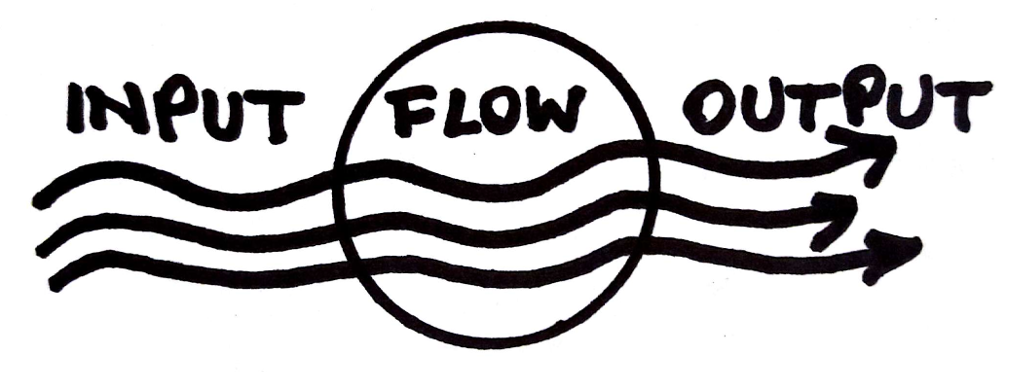
\includegraphics[width=0.50\textwidth]{FlowSystem}
  \caption{Sistema fluyente}
  \centering
  \label{fig:FlowSystem} %\ref{fig:FlowSystem}
\end{figure}

Las habilidades y las destrezas de un equipo, como de sus integrantes, deben estar en equilibrio con el reto de lo que se tiene que hacer. Cuando eso se logra, se alcanza una armonía de un proceso fluyente, con ritmo, con cadencia. Cuando se habla de cadencia se refiere a esta idea de fluir con ritmo. Desde un punto de vista sistémico, equivale a decir que debe existir cierta relación proporcional y estable entre el promedio de la tasa de entrada al sistema con el promedio de la tasa de salida (promedio de la velocidad), en relación al tiempo. Para que ocurra el sistema debe comportarse como un flujo de trabajo con personas jalando tareas a un ritmo sostenible y armónico. Y para fluir con ritmo es necesario limpiar el proceso, es decir, hacerlo magro: eliminar desperdicios, diluir problemas, mitigar riesgos, evadir obstáculos, etcétera. Un líder de Scrum es un facilitador, alguien que facilita el flujo. Y para facilitar el flujo es necesario, entre otras cosas, disciplina. El marco Scrum es el marco disciplinario que encauza el flujo.

